\chapter{Experiment}
\label{ERef}
Er hebben doorheen het jaar, verschillende experimenten plaats gevonden. We zijn begonnen met meer eenvoudige experimenten en zijn geeindigd met de moeilijkere experimenten. We bespreken de experimenten in chronologische volgorde. Na de beschrijving en de uitwerking van de verschillende experimenten worden conclusies getrokken uit de resltaten en de berekeningen. Met de conclusies van de vorige experimenten werd dan ook rekening gehouden bij de uitvoering van de volgende experimenten. Er zijn vier verschillende experimenten gebeurd. We beginnen met opslaan van beelden \ref{ERefOvB}. Vervolgens detecteren we het uit het bed stappen \ref{ERefDUB}. Dit deel is opgeslitst in twee verschillende experimenten, nameelijk een eerst poging \ref{ERefDUBEP} en een tweede poging \ref{ERefDUBTP}. Als laatste experiment werken we met live beelden \ref{ERefELB}.

\section{Opslaan van beelden}
\label{ERefOvB}
Dit eerste experiment bespreken we in 4 verschillende delen. We beginnen met te verklaren wat ons doel was van het experiment \ref{ERefOBD}, daarna bespreken we de gebruikte klassen, methodes en het flowchart \ref{ERefOBF}. Vervolgens verklaren we de specifieke uitwerking van het experiment \ref{ERefOBU}. Als laatste trekken we onze conclusies \ref{ERefOBB}.

\subsection{Doel van het experiment}
Het doel van dit experiment is het opslagen van beelden. Dit om dan achteraf verschillende processen over de beelden te laten lopen en zo te zien welke de beste resultaten geeft.
\label{ERefOBD}

\subsection{Gebruikte klassen en flowchart}
\label{ERefOBF}
Voor dit expermiment werd voornamelijk de gekregen code geruikt om de code met de computer in te lezen. Vervolgens maken we gebruik van de klassen SaveImages \ref{mRefSIm}, GetImages \ref{mRefGIm} en Detect \ref{mRefDet}. De opeenvolging van de gebruikte methodes vindt u terug in de flowchart. 

\subsection{Uitvoering experiment}
\label{ERefOBU}
\begin{figure}[h]
	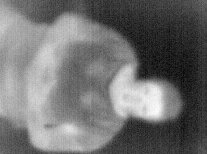
\includegraphics[scale=0.65]{EersteExperiment_img0}
	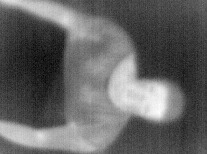
\includegraphics[scale=0.65]{EersteExperiment_img2}
	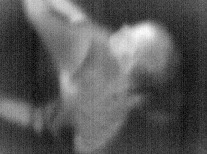
\includegraphics[scale=0.65]{EersteExperiment_img3}
	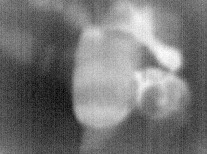
\includegraphics[scale=0.65]{EersteExperiment_img6}
	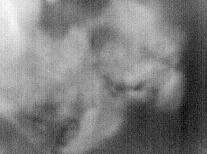
\includegraphics[scale=0.65]{EersteExperiment_img9}
	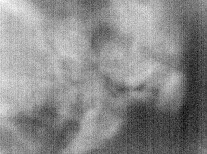
\includegraphics[scale=0.65]{EersteExperiment_img10}
	\caption{Opgeslagen beelden in eerste experiment}
	\label{imgEEx}
\end{figure}
Tijdens het eerste experiment hebben we overdag met behulp van de camera \ref{mRefSTh} beelden genomen van een persoon in bed. Hiervoor gebruiken we voornamelijk de klasse SaveImages \ref{mRefSIm}. Al gaan we hier maar om de 50 frames opslaan. Deze beelden kunnen we dan gebruiken voor het maken van bijvoorbeeld het masker en het verder afwerken van de detectie. Verder hebben we tijdens het maken van de beelden er ook op gelet dat de persoon verschillende slaaphoudingen aannam. Zo kunnen we nagaan of er een goede segementatie gebeurde vooralleer we begonnen met het maken van beelden gedurende een volledige nacht.\\
De beelden die zijn opgeslagen tijdens dit eerste experiment vindt u terug in figuur \ref{imgEEx}. Zoals u ziet hebben we zoveel mogelijk verschillende slaaphoudingen aangenomen. We zien eveneens een verschil in de afbeeldingen bij gebruik van een deken. De twee laatste afbeeldingen zijn van het leeg bed net nadat de foto's gertokken zijn. \\
Tijdens dit experiment hing de camera boven het bed. Een schets van het zijaanzicht van de situatie vindt u in afbeelding \ref{imgEEx2}. De oranje rechtoeken zijn de muren, plafond en grond van de kamer. Het paarse driehoekje is de camera. De camera hing boven het hoofdeinde van het bed, ongeveer in het midden van de breedte van het bed. \\
\begin{figure}[h]
	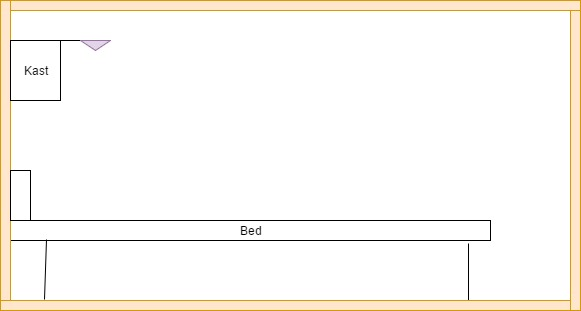
\includegraphics[scale=0.5]{SchetsExperiment1}
	\caption{Schets van de situatie in het eerste experiment}
	\label{imgEEx2}
\end{figure}
De foto's werden opgeslagen in de gewenste map. Verder zien we dat de persoon duidelijk te scheiden is van de achtergrond. Alleen zouden we de camera verder van het bed moeten plaatsen om meer van het bed op de beelden te kunnen zien. Door gebruik te maken van deze afbeeldingen, zochten we ook naar de ideale waarde voor de drempelwaarde om het masker te cre\"eren, zoals reeds besproken is bij de verschillende methodes van de klasse Detect \ref{mRefDet}.

\subsection{Besluiten uit het experiment}
\label{ERefOBB}
 Bij het bekijken van de opgeslagen beelden \ref{imgEEx} viel er ons iets op. Als er een deken over de persoon ligt, was hiervan enkel nog het hoofd en eventueel ook armen zichtbaar. Verder warmt het bed zeer snel op. Zo kan je in de laatste frames een leeg bed zien nadat de persoon er voor ongeveer 10 minuten had ingelegen. Dit is ook al zeer licht en kan leiden tot valse persoon detecties, dit is natuurlijk niet wenselijk voor ons experiment. Hiervoor gaan we dus in de komende experimenten een oplossing moeten zoeken. Het resultaat van het verkregen masker, vindt u in figuur \ref{imgCOB}.
\begin{figure}[h]
	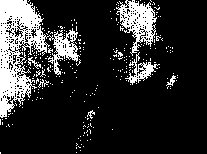
\includegraphics[scale = 0.75]{EersteExperiment_mask10}
	\caption{Verkregen masker voor leeg opgewarmd bed}
	\label{imgCOB}
\end{figure}
Ook ziet u dat als de persoon eerst op de zij heeft gelegen en gedraaid is een lichter vlak op de plaats waar de persoon voordien lag.
Een tweede mogelijk probleem dat optreedt is dat als je het masker cre\"eert, je de lichaamsdelen die bedekt worden door een deken maar ook door bijvoorbeeld een kledingstuk zoals pyama soms mist. Hierdoor zou het kunnen dat mogelijke aanstalten om uit het bed te stappen niet gedetecteerd worden. \\
Verder maakt de camera ook een klikgeluidje elke keer als er een frame gemaakt wordt. Dit kunnen sommige mensen hinderlijk vinden als ze hier mee moeten slapen. Dit kan enkel opgelost worden door een andere camera te gebruiken.  

\section{Detecteer uit bed stappen}
\label{ERefDUB}
Net zoals bij het voorgaande experiment \ref{ERefOvB} bespreken we ook dit tweede experiment in drie verschillende delen. We beginnen met het doel van het experiment \ref{ERefDBD} en het verduidelijken van de gebruikte klassen en methodes \ref{ERefDBK}. Vervolgens verklaren we de uitwerking \ref{ERefDBV} en als laatste nemen we een paar besluiten uit de verkregen beelden \ref{ERefDBB}. 

\subsection{Doel van het experiment}
\label{ERefDBD}
Het doel van het experiment is te bepalen of het mogelijk is te detecteren wanneer een person uit bed stapt. En het ontwikkelen van de algoritmes die hiervoor nodig zijn. 

\subsection{Gebruikte klassen en flowchart}
\label{ERefDBK}
Er wordt hier verder gebouwd op het voorgaande experiment \ref{ERefOvB}. Daarom maken we gebruik van dezelfde drie klassen, namelijk: SaveImages \ref{mRefSIm}, GetImages \ref{mRefGIm} en Detect \ref{mRefDet}. Hiernaast wordt tijdens dit experiment ook gebruik gemaakt van de klasse Bed \ref{mRefBed}. Het flowcharts van de experimenten zoals weergegeven in figuur \ref{imgFCDUBEP} en figuur \ref{imgFCDUBTP} tonen de opeenvolging van de gebruikte methodes.

\subsection{Verklaring uitwerking van het experiment}
\label{ERefDBV}
\begin{figure}[h]
	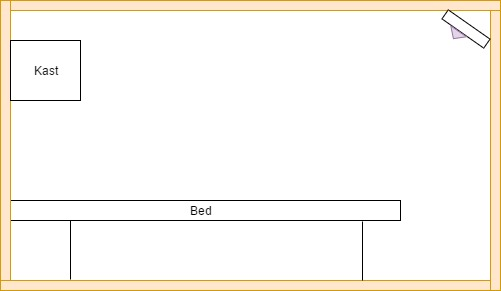
\includegraphics[scale=0.6]{SchetsExperimentTwee}
	\caption{Schets van het tweede experiment}
	\label{imgTEx}
\end{figure}
Eens de persoon uit de beelden gehaald kon worden. Hebben we nieuwe beelden gemaakt. Dit waarbij de hoeken van het bed gedefinieerd werden door middel van de constructor met een afbeelding \ref{mRefBed}. Daarna maakte de persoon verschillende keren aantstalten om uit het bed te stappen en hebben we nagegaan dat ons programma de juiste kant kan detecteren. \\
Voor dit experiment werd een nieuwe opstelling gemaakt. Een schets hiervaan vindt u in figuur \ref{imgTEx}.
Ook in deze figuur \ref{imgTEx} zijn de oranje rechthoeken de muren, plafond en vloer. De camera is eveneens het paarse driehoekje. We voegen eveneens een paar voorbeelden toe van gemaakte beelden tijdens dit experiment, deze kan u zien in figuur \ref{imgTEx1}.
\begin{figure}[h]
	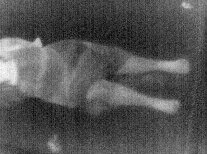
\includegraphics[scale=0.85]{TweedeExperiment_img0}
	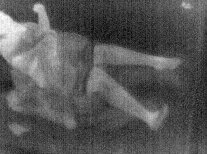
\includegraphics[scale=0.85]{TweedeExperiment_img4}
	\caption{Voorbeelden van opgeslagen afbeeldingen tijdens tweede experiment}
	\label{imgTEx1}
\end{figure}
Dit experiment is op twee verschillende manieren uitgevoerd. Dit omdat we niet tevreden waren met de resultaten die we de eerste keer verkregen. We bespreken eerst de eerste poging en vervolgens de tweede poging. 
\subsubsection{Eerste poging}
\label{ERefDUBEP}
\begin{figure}[h]
	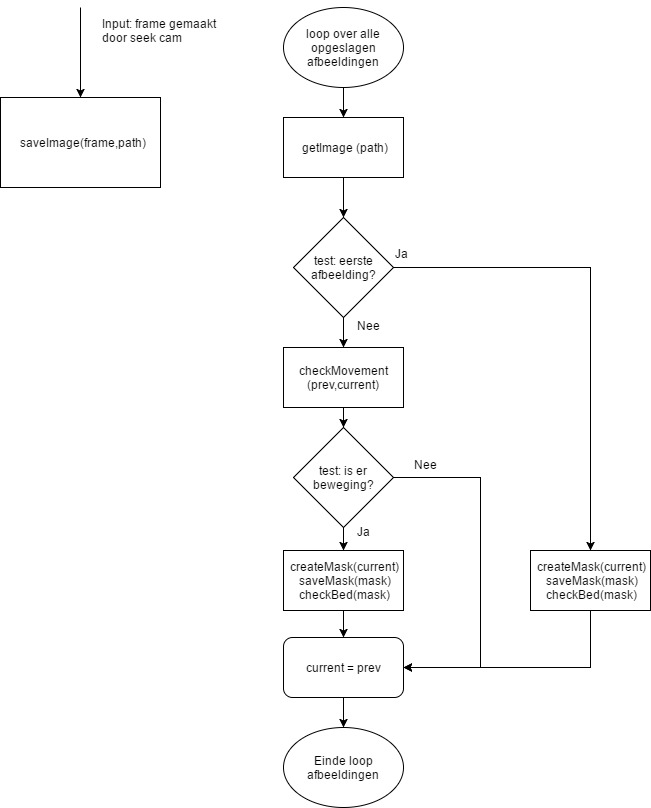
\includegraphics[scale=0.45]{FlowChart_DetectUitBed_EerstePoging}
	\caption{Flowchart eerste poging detectie uit bed stappen}
	\label{imgFCDUBEP}
\end{figure}
Om het idee achter dit experiment te verduidelijken, voegen we een flowchart toe met daarin de gebruikt methodes om tot onze resultaten te komen, dit flowchart vindt u terug in figuur \ref{imgFCDUBEP}. We houden hier wel rekening met beweging om rekentijd de besparen. Maar we controleren nergens of de oppervlakken in het masker die het alarm gaan triggeren wel bewegende delen zijn of onderdelen van de achtergrond. De gebruikte methodes worden allemaal besproken in de sectie code \ref{mrefCod}

\subsubsection{Tweede poging}
\label{ERefDUBTP}
\begin{figure}[h]
	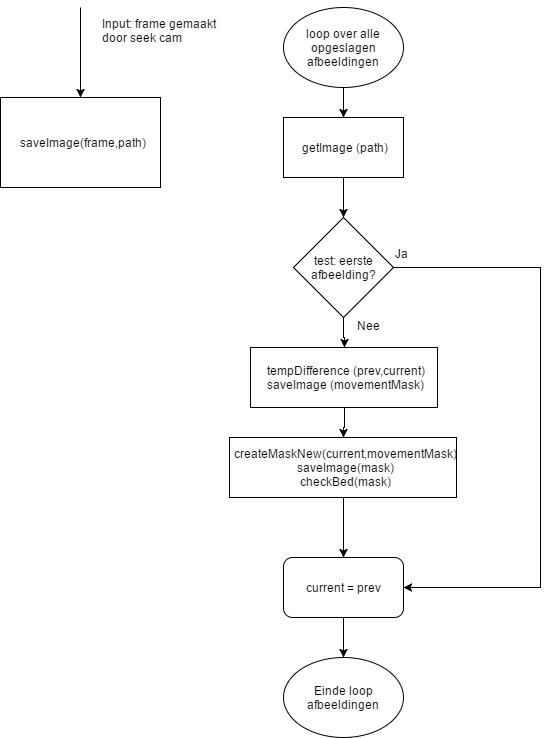
\includegraphics[scale=0.45]{FlowChart_DetectUitBed_TweedePoging}
	\caption{Flowchart tweede poging detectie uit bed stappen}
	\label{imgFCDUBTP}
\end{figure}
Nadat we onze conclusies hebben getrokken uit de eerste poging van ons experiment \ref{CRefDUBEP}, hebben we onze code aangepast. Het flowchart van deze aanpassingen vindt u in figuur \ref{imgFCDUBTP}. Het grootste verschil is dat we hier een temporeel verschil berekenen. Dit wordt opgeslagen als bewegingsmasker. Hierdoor gaan warme punten in de achtergrond, het alarm niet meer triggeren. De gebruikte methodes worden besproken in \ref{mrefCod}.

\subsection{Besluiten na de experimenten}
\label{ERefDBB}
In dit bespreken we de conclusies die we hebben getrokken uit het detecteren van het uit bed stappen. De conclusie over dit stukje wordt in twee delen gesplitst. Dit omdat de resultaten van de geruikte code in het eerste deel niet volstaat, daarna hebben we een paar aanpassingen in onze code gemaakt, de conclusies die we trekken na het toepassen van deze nieuwe code wordt als laatste besproken.

\subsubsection{Eerste poging}
Bij het bekijken van de resultaten van het tweede experiment, valt bij het maken van de maskers op dat er een lichtere vlek (rechtsbovenaan), ook mee gedetecteerd wordt, dit is echter geen deel van een persoon. De maskers ziet u in figuur \ref{imgCDUB}.
\begin{figure}[h]
	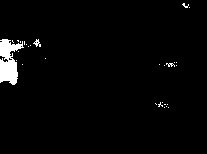
\includegraphics[scale = 0.75]{MaskTweedeExperiment_img0}
	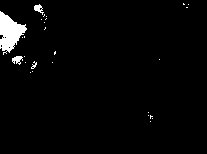
\includegraphics[scale = 0.75]{MaskTweedeExperiment_img4}
	\caption{Verkregen masker voor twee voorbeelden bij experiment twee}
	\label{imgCDUB}
\end{figure}
Hierdoor krijgen we steeds de melding dat de persoon uit het bed probeert te stappen langs de rechterzijde. Dit is natuurlijk een fout. Een mogelijke oplossing voor dit probleem is eerst detecteren welke pixels verandert zijn, daar is dus een beweging. Vervolgens kunnen we voor de bewogen pixels kijken welke warm genoeg zijn om tot de persoon te behoren. Zo kunnen we deze valse detecties vermijden. Hierdoor gaat de computer wel veel meer moeten rekenen.

\subsubsection{Tweede poging}
Nadat we eerst het temporeel verschil berekenen voor we het masker maken van de lichaamswarmte op de infraroodbeelden, kunnen we door gebruik te maken van de setSidesOfBed methode van de klasse Bed bepalen langs welke kant de persoon uit het bed probeerd te stappen. Als de persoon binnen de randen van het bed blijft wordt er None terug gegeven. Indien de randen van het bed wel wordt overschreven, wordt links of rechts (naargelang langs welke kant de rand wordt overschreven) afgedrukt op het scherm. Uit deze tweede poging van dit experiment kunnen we besluiten dat de detectie van langs welke zijde de persoon uit het bed stapt correct werkt. Het meten van de tijd dat een persoon weg blijft, is momenteel nog onmogelijk door de restwarmte die we nog zien in onze beelden. Een mogelijke oplossing hiervoor wordt in een volgend experiment aangeboden. 

\section{Experiment met live beelden}
\label{ERefELB}
De totale bespreking van het experiment op live beelden wordt uit gelegd in drie verschillende delen. We beginnen met te verklaren wat het doel \ref{ERefLBD} van dit experiment was, hierna bespreken we de opbouw en de uitwerking van het experiment \ref{ERefLBV}. Als laatste bespereken we de besluiten die we trekken uit dit experiment. 

\subsection{Doel van het experiment}
\label{ERefLBD}
Het doel van dit experiment is na te gaan of we de veranderingen in de beelden snel genoeg detecteren. We gaan dus testen of de detectie van langs welke zijde er aanstalten gemaakt worden om uit bed te stappen ook ogenblikkelijk gebeuren. 

\subsection{Uitwerking van het experiment}
\label{ERefLBV}
We  hebben ons systeem aangesloten op de camera en live beelden verwerkt. De proefopstelling is het zelfde gebleven als bij het vorige experiment \ref{ERefDUB}. Een schets hiervan ziet u in figuur \ref{imgTEx}. Tijdens dit experiment is er een persoon in het bed gaan liggen en heeft een paar keer gedaan als hij uit het bed wou stappen. Terwijl op het scherm in het oog werd gehouden of de computer de juiste detecties werden gemaakt.

\subsection{Besluiten na het experiment}
 Uit dit experiment kunnen we besluiten dat het systeem werkt. Vanaf er een arm of een been uit het bed wordt gestoken wordt er een melding gegenereerd met de juiste zijde. Het genereren van deze melding gebuerd vrijwel onmiddelijk. Kleding en deken vormt hier nog het grootste probleem. Als het lichaam bedekt is, wordt het door het masker niet gedetecteerd. Hierdoor zouden er evenementen gemist kunnen worden. Verder loopt het ook mis als er een persoon in het bed heeft gelegen en er uit stapt. De camera detecteerd dan de restwarmte an het bed en gaat doen alsof er wel nog een persoon in ligt. Zoals reeds eerder is aangehaald, wordt hiervoor in een volgende experiment een oplossing gezocht. 


\chapter{Algemeen besluit}
Het systeem detecteerd goed langs welke zijde er uit het bed gestapt wordt. Een mogelijk uitbereiding is de timer van hoelang een persoon uit bed is. Momenteel lukt dit nog niet door de restwarmte van het bed. Indien er ook wenst gewerkt te worden zonder de afbeeldingen op te slagen moet er ook nog aan de code gewerkt worden. De beelden die door de camera worden geleverd staan in een ander formaat als de beelden die ik verwerk, bijgevolg moeten er dan nog een paar kleine aanpassingen gebeuren. Verder kan er ook nog onderzoek gebruiken naar het gebruik van een night vision camera, om het probleem van de restwarmte te verkleinen. Verder kunnen ook andere cameras eens getest worden, de meeste mensen klagen over het klikgeluidje dat de camera maakt.